\documentclass[authoryear]{elsarticle}
\usepackage{latexsym}
%\usepackage{rotate}
\usepackage{graphics}
\usepackage{amsmath}
\usepackage{amssymb}
\usepackage{comment}
\bibliographystyle{chicago}



\newcommand{\logit}{\mathrm{lgt}}
\newcommand{\I}{\mathrm{I}}
\newcommand{\E}{\mathrm{E}}
\newcommand{\p}{\mathrm{P}}
\newcommand{\e}{\mathrm{e}}
\newcommand{\vecm}{\mathrm{vec}}
\newcommand{\kp}{\otimes}
\newcommand{\diag}{\mathrm{diag}}
\newcommand{\cov}{\mathrm{cov}}
\newcommand{\eps}{\epsilon}
\newcommand{\ep}{\varepsilon}
\newcommand{\obdots}{\ddots}    % change this later
\newcommand{\Ex}{{\cal E}}
\newcommand{\rat}{{\frac{c_{ij}}{c_{i,j-1}}}}
\newcommand{\rmu}{m}
\newcommand{\rsig}{\nu}
\newcommand{\fd}{\mu}
\newcommand{\tr}{\mathrm{tr}}
\newcommand{\cor}{\mathrm{cor}}
\newcommand{\bx}[1]{\ensuremath{\overline{#1}|}}
\newcommand{\an}[1]{\ensuremath{a_{\bx{#1}}}}

\newcommand{\bi}{\begin{itemize}}
\newcommand{\ei}{\end{itemize}}

\renewcommand{\i}{\item}
\newcommand{\sr}{\ensuremath{\mathrm{SRISK}}}
\newcommand{\cs}{\ensuremath{\mathrm{CS}}}
\newcommand{\cri}{\ensuremath{\mathrm{Crisis}}}
\newcommand{\var}{\ensuremath{\mathrm{VaR}}}
\newcommand{\covar}{\ensuremath{\mathrm{CoVaR}}}
\newcommand{\med}{\ensuremath{\mathrm{m}}}
\newcommand{\de}{\mathrm{d}}
\renewcommand{\v}{\ensuremath{\mathrm{v}_q}}
\newcommand{\m}{\ensuremath{\mathrm{m}}}
\newcommand{\tvar}{\ensuremath{\mathrm{TVaR}}}
\renewcommand{\c}{\ensuremath{\mathrm{CoVaR_q}}}
\renewcommand{\v}{\ensuremath{\mathrm{VaR}_q}}



\newcommand{\eref}[1]{(\ref{#1})}
\newcommand{\fref}[1]{Figure \ref{#1}}
\newcommand{\sref}[1]{\S\ref{#1}}
\newcommand{\tref}[1]{Table \ref{#1}}
\newcommand{\aref}[1]{Appendix \ref{#1}}




\newcommand{\cq}{\ , \qquad}
\renewcommand{\P}{\mathrm{P}}
\newcommand{\Q}{\mathrm{Q}}

\newcommand{\Vx}{{\cal V}}
\newcommand{\be}[1]{\begin{equation}\label{#1}}
\newcommand{\ee}{\end{equation}}




\begin{document}

% Title of paper
\title{Systemic risk and contagion effects in Australian financial institutions and sectors}
% List of authors, with corresponding author marked by asterisk
\author{Piet de Jong,  Geoff Loudon and Weihao Choo \\[4pt]
% Author addresses
\textit{Department of Applied Finance and Actuarial Studies\\ Macquarie University, Sydney, NSW 2109.}
\\[2pt]
%E-mail address for correspondence
{piet.dejong@mq.edu.au}}

% Running headers of paper:
\markboth%
% First field is the short list of authors
{De Jong}
% Second field is the short title of the paper
{Systemic risk}

\begin{abstract}
This article refines, builds on and extends  SRISK methodology recently proposed in the literature.  The refinement is to define SRISK in terms of a put on the Basel shortfall.   The definition is built on by defining the systemic beta of a firm in terms of the departure of a stressed expectation from the normal expectation the put.  By stressed expectation is meant an expectation that averages conditional expectations over outcomes defined by a stressor variable combined with  a stressor function.  The stressor variable and function are chosen by the practitioner and include functions of a  market wide variable. Since stressed expectations are linear, a system systemic beta is naturally defined as linear in the firm specific systemic beta's.    The methodology  generalises automatically to situations where systemic stress arises from the interaction of multiple system wide variables.    Application is made to Australian financial data. 
\end{abstract}

\maketitle

\section{Literature review}

The starting point for the proposed research is the recent literature and the CIFR targeted areas and APRA aims and functions.
This recent literature includes the following
\cite{adrian2011covar},
\cite{acharya2012capital},
\cite{acharya2012measuring}
and \cite{brownlees2010volatility}.   The proposed research aims to extend and apply these techniques particularly in relation to the entities regulated by APRA.   Thus our  broad aim is to develop, implement and bring to bear recent developments in stress testing  on the aims of APRA and the CIFR targeted research areas detailed above.   




\section{Capital shortfall and leverage}

If $d_{it}$ and $w_{it}$ are the debt and equity of a firm $i$ at time $t$ and $k$ is the capital requirement,  then the capital shortfall at time $t$ is 
\be{shortfall}
k(d_{it}+w_{it}) - w_{it} = kd_{it}  - (1-k) w_{it} = kd_{it}\left(1-\e^{-\ell^*_{it}}\right)\ ,
\ee
where 
$$
\ell_{it} \equiv \ln\frac{d_{it}}{w_{it}}\cq \ell_{it}^* \equiv \ell_{it} + \logit\ k \cq \logit\ k\equiv \ln \frac{k}{1-k} \ .
$$
The quantity $\ell^*_{it}$ is called Basel adjusted the log--leverage and $\ell^*_{it}>0$ implies capital shortfall \eref{shortfall} is positive. 


Basel II assumes $k=0.08$ implying $\logit(k)=-2.44$,  $\ell_{it}^*=\ell_{it}-2.44$  and there is  positive  ``Basel shortfall"  if
$\ell^*_{it}>0$ or $\ell_{it} > 2.44$.
As the log leverage $\ell_{it}$  increases to 2.44 the firm approaches the Basel II threshold. 

\fref{Bloglev} displays Basel log--leverages for the four major and four minor Australian banks listed in \tref{banks} on the first trading day of each month from January 2003  through to December 2014.  Note most banks are Basel compliant up to about 2008.

\begin{figure}[htbp]
\begin{center}
\label{Bloglev}
\includegraphics{Bloglev.pdf}
\caption{Basel log--leverages for four major (left panel) and four minor (right panel) Australian banks from 2003 through to end of 2014.  Note all banks contravene the Basel II threshold (corresponding to Basel log-leverage of 0) on or around the early part of 2009.}
\end{center}
\end{figure}


\section{Future capital shortfall}

Financial institutions and regulators are concerned with future Basel compliance and understanding  the likelihood of a  future Basel breach.   Future compliance depends on the future return on equity.   Consider  firm $i$ at time  $t+h$ where $h>0$.  Then
$$
\ell_{i,t+h} = \ln \frac{d_{i,t+h}}{w_{i,t+h}} = \ell_{it} -\nu_{it}\cq \nu_{it}\equiv \ln\frac{w_{i,t+h}}{w_{it}}  \ ,
$$
where it is assumed $d_{i,t+h}=d_{it}$.  Hence $\nu_{it}$ is the return on equity over $(t,t+h)$.  The future return is unknown at time $t$ but may be its distribution may be  well understood.

In terms of the Basel leverage $\ell_{it}^*$ at time $t$, the  Basel II shortfall  at time $t+h$ is,
\be{bs}
d_{it}k(1-\e^{\nu^*_{it}})\cq \nu_{it}^*\equiv \nu_{it}-\ell^*_{it}=\nu_{it}-\ln\frac{d_{it}}{w_{it}}-\logit\ k\ . 
\ee 
The Basel II limit is reached at $t+h$ if $\nu_{it}=\ell_{it}^*$ ($\nu_{it}^*=0$) and  breached  if
$
\nu_{it}< \ell_{it}^*
$ ($\nu_{it}^*<0$).
A breach is  unlikely if $\ell^*_{it}$ is low i.e. either the log--leverage is low, or the Basel constant $k$ is low.
\newcommand{\Es}{\E_\phi}





\section{Systemic risk -- SRISK}

\cite{brownlees2015} define the systemic risk (SRISK) of a group of firms  at time $t$ as
\be{esrisk}
k\sum_i d_{it}|1-\Es(\e^{\nu^*_{it}})|^+  \ ,\ \ |x|^+\equiv \max(0,x)\ ,\ \  \nu_{it}^*\equiv \nu_{it}-\ln\frac{d_{it}}{w_{it}}-\logit\ k\ ,
\ee
where $k$ is the Basel constant, $d_{it}$  and $\nu^*_{it}$ are, respectively,  the debt and the Basel and log--leverage adjusted future return  of firm $i$ at time $t$,  and $\Es$ denotes  expectation conditional on a stress event $\phi$:  in their case a severe general market downturn.
The contribution of firm $i$ is thus a put on the conditional expected value of the Basel II shortfall of firm $i$ at $t+h$.

 The proportionate contribution of firm $i$  to \eref{esrisk} is called the systemic risk of firm $i$:
 \be{sriskperc}
 \mathrm{SRISK}_i\equiv\frac{|1-\Es(\e^{\nu^*_{it}})|^+}{\Ex\{|1-\Es(\e^{\nu^*_{it}})|^+\}}\ , 
 \ee
where $\Ex$ denotes  debt weighted averaging.     A large $\mathrm{SRISK}_i$ indicates a systemically important firm.  The  expression \eref{sriskperc} depends on $k$ only through its logit.  The values of the ``puts" $|1-\Es(\e^{\nu^*_{it}})|^+$  in \eref{sriskperc} are known at time $t$:  there is no uncertainty except for possible estimation uncertainty in the stressed expected value.

 If the stressed distribution of $\nu^*_{it} $ is concentrated on the negative axis then  $\e^{\nu^*_{it}}<0$ and
$$
|1-\Es(\e^{\nu^*_{it}})|^+ =\Es(|1-\e^{\nu^*_{it}}|^+)\ .
$$
If, under stress, the probability of $\nu^*_{it}>0$ is positive  then the last relation only holds approximately.   The SRISK contribution of a firm is zero whenever
\be{cond}
\Es(\e^{\nu^*_{it}})\equiv \e^{-\ell_{it}^*}\Es(\e^{\nu_{it}})\le 1\cq \ln \Es(\e^{\nu_{it}})\le\ell^*_{it}\equiv\ln\frac{d_{it}}{w_{it}}+\logit(k)\ .
\ee
This inequality often holds even if the expectation is severely stressed.  In particular if the stressed distribution of $\nu_{it}$ is normal with mean $\mu$ and variance $\sigma^2$ then
$$
\ln \Es(\e^{\nu_{it}}) = h\mu +h^2\frac{\sigma^2}{2}\ ,
$$
and  \eref{cond} is equivalent to
$$
\mu +h\frac{\sigma^2}{2}\le \frac{\ell_{it}^*}{h} \ ,
$$
indicating a Basel breach is unlikely if $\ell^*_{it}$ is very negative equivalent to  $\ell_{it}$ well below 2.44, the Basel limit.


The system SRISK is zero if all firm the SRISK contributions are zero that is if \eref{cond} holds for every $i$.  This would be usual in the Australian case.



An improvement is where firms with capital surplus are included, since they, especially those with large surpluses, are systemically important but in a positive way by dampening the impact from distressed firms.  Second, it is  appropriate to consider the departure from the unconditional expectation to differentiate firms which only experience capital shortfall during a market downturn as opposed to those who already have large shortfalls in average conditions.   This leads to the revised computation
$$
\frac{1-\Es(\e^{\nu^*_{it}})-\{1-\E(\e^{\nu^*_{it}})\}}{\Ex\{|1-\Es(\e^{\nu^*_{it}})|^+-|1-\Es(\e^{\nu^*_{it}})|^+\}} = \frac{\E(\e^{\nu^*_{it}})-\Es(\e^{\nu^*_{it}})}{\Ex\{|1-\Es(\e^{\nu^*_{it}})|^+-|1-\Es(\e^{\nu^*_{it}})|^+\}} 
$$


The revised contribution of firm $i$ to total systemic risk is hence
$$
\frac{\mathrm{SRISK}_i-\E(c_i)}{\mathrm{SRISK}_m-\E(c_m)}
=\frac{w_i }{w_m } \frac{\E(r_i)-\E(r_i|u_m<a)}{\E(r_m)-\E(r_m|u_m<a)} \;,
$$
the product of the equity of firm $i$ relative to total market equity and return movement of firm $i$ in a market downturn relative to overall market movement.

\section{Improved systemic risk measurement}

For  firm $i$ define the  Basel put and  Basel risk as 
\be{put}
p_{it}\equiv k |1-\e^{\nu^*_{it}}|^+\cq \E(p_{it})\ge 0\ ,
\ee
where $\E$ denotes normal or unstressed expectation.  The Basel risk in firm $i$ depends only $k$,  the present leverage,  and the lower tail of the  $\nu_{it}$ distribution.  The put value \eref{put} is stated in terms of unit debt and increases with $k$, both directly from  multiplication by $k$ and indirectly through its logit, making a positive put outcome more likely.  

Default put options similar to \eref{put} have been discussed in the insurance literature as critical to an evaluation of a firm:  see for
example \citet{merton1977analytic}, \citet{doherty1986price}, \citet{cummins1988risk}, \citet{myers2001capital} and \citet{sherris2006solvency}.

The total Basel put value and hence Basel risk for firm  $i$ is   $d_{it}\E(p_{it})$.   This is the cost of insuring firm $i$ does not breach the Basel standard.  In practice it may be appropriate to discount $p_{it}$ in \eref{put} by the interest rate over the period $(t,t+h)$ and value the put with risk neutral rather than normal expectation.       

The put $p_{it}$ is tradable since, given $k$, it relies only on the present leverage and the future return $\nu_{it}$ on equity $w_{it}$.  Market participants can value the put in  the same way as any other put and use the contract to diversify risk.  Firms can buy puts in the market to hedge Basel default risk.    

However regulators will value the puts $p_{it}$ using a stressed, rather than risk neutral, expectation.   Stressed expectations correspond closely to conditional expectation given a systemically important event or events.    Regulators are concerned with the possibility of Basel breaches if such events occur and hence have an overbearing interest in monitoring stressed expectations.   In the extreme regulators can charge firms all or a  proportion of their stressed put values if there are implicit government bailout guarantees.

In terms of the put values $\E(p_{it})$, the  system Basel risk is defined as the debt weighted average of the individual firm's put values:
\be{nsrisk}
\Ex\{\E(p_{it})\} = \E\{\Ex(p_{it})\}  \ , 
\ee
since both $\E$ and $\Ex$ are linear.
The  system Basel risk is stated per unit of system debt.  The dollar value of Basel risk is the Basel risk multiplied by the total system debt:
$$
d_t\Ex\{\E(p_{it})\}  = \sum_id_{it}\E(p_{it}) \cq d_t\equiv\sum_id_{it}\ .
$$
Thus the monetary  Basel risk is a  weighted average  of firm specific monetary Basel risks.  




\section{Systemic stress as stressed expectation}

In the above development $\E$  denotes  unstressed expectation:  that is expectation that does not assume a stressful scenario.   A stressed expectation, denoted $\Es$, is a
linear combination of  expectations, each assuming some level of stress
\be{formula}
\Es(p_{it}) \equiv \E\{\phi\E(p_{it}|\phi)\} = \E(\phi p_{it}) = \E(p_{it}) + \cov\{\E(p_{it}|\phi),\phi\}\ .
\ee 
Here $\phi\ge 0$ with $\E(\phi)=1$ is thought of as a stress factor or ``stressor,"  defining events impacting $p_{it}$  and serving as a basis for stress testing.  Thus $\phi$--stressing  changes the expected value $\E(p_{it})$ by the covariance between the conditional expectation $\E(p_{it}|\phi)$  and the stressor $\phi$.

The conditioning variable $\phi$  downplay or highlight different scenarios.  The conditioning events are scenarios of interest and  probabilistic weighting is according to the level of interest.  The first equality in \eref{formula}  from the definition of conditional probability \citep{whittle2000probability}.  The second equality follows from
$$
\cov(p_{it},\phi)=\cov\{\E(p_{it}|\phi),\phi\}\ .
$$
The covariance is zero whenever  $p_{it}$ is independent of $\phi$ which occurs if $\phi=1$.

  To a Bayesian the stressed expectation \eref{formula}  is the mean of $p_{it}$  in  the posterior density
\be{post}
\int \phi f(p_{it}|\phi) f(\phi)\de \phi=\int \phi f(p_{it},\phi)\de \phi= \E(\phi|p_{it})f(p_{it})\ .
\ee
Note \eref{post} is a density since $\phi\ge 0$ and $\E(\phi)=1$.   Any outcome $p_{it}$ such that $\E(\phi|p_{it})$ is large  is amplified and vice versa.   Further
$$
\E_s(p_{it})  = \E\left\{p_{it} \frac{\phi f(p_{it})}{f(p_{it})}\right\}\ ,
$$
that is the density  $f(p_{it})$ of $p_{it}$  is replaced by  the density $\phi f(p_{it})$.  Hence more importance is given to those outcomes given more weight by $\phi$. 


\section{Systemic beta's}
Writing  $\sigma_{\phi}$ as the standard deviation of $\phi$,  define the systemic beta of firm $i$ with respect to stress $\phi$ as
\be{zscore}
\beta_{it}\equiv \frac{\Es(p_{it})- \E(p_{it})}{\sigma_\phi}= \frac{\E\{(\phi-1)p_{it}\}}{\sigma_\phi}= \frac{ \cov\{\E(p_{it}|\phi),\phi\}}{\sigma_\phi} \cq
\ee
where  $\sigma_\phi$ is the standard deviation of $\phi$.  Thus
\be{zscore2}
\Es(p_{it}) = \E(p_{it}) + \beta_{it}\sigma_\phi\cq \E(p_{it}|\phi) \approx \E(p_{it}) + \beta_{it}\frac{\phi-1}{\sigma_\phi}\ .
\ee
The second, approximate, relationship is suggested from  a regression interpretation of $\cov(p_{it},\phi)/\sigma^2_\phi$ as the regression coefficient of $p_{it}$ on $\phi$.

The formulas in \eref{zscore2} suggests two ways of  thinking about the  systemic beta's  $\beta_{it}$.   First, the left hand side equation shows systemic stress $\beta_{it}$ serves to shift the mean of put prices  by, on average, $\sigma_\phi$.   The shift $\beta_{it}\sigma_\phi$ is the market price of stress embedded in firm $i$ at time $t$.   Firms with large shifts embody stress risky firms.

The second interpretation is based on  the right hand side approximation in \eref{zscore2} showing   the change in the  expected Basel put price if  $\sigma_\phi$ units of stress $\phi$ are applied.  The quantity $(\phi-1)/\sigma_\phi$ is thought of as a ``stress factor."   The stress factor has mean 0 and standard deviation 1 and is scaled by $\beta_{it}$ to yield the actual stress effect on  $p_{it}$.  Thus  $\beta_{it}$ is thought of a usual finance type ``beta" with respect to the given $\phi$.   Stress is measured in standardised units.  Units of stress take on different meaning depending on  $\phi$ as discussed below. The distribution of $\phi$ determines the distribution of the stress factor. If the stress factor is normally distributed then a stress effect more than doubling of the put value  occurs less than about $2.5\%$ of the time. 

Note the systemic beta's are stated in terms of additions to the normal put price $\E(p_{it}$. Thus in an increasingly dire financial situation $\E(p_{it})$ will increase.   However stress $\beta_{it}$ measures the  change in current put values  under  further $\phi$--stress.  This varies from  \cite{brownlees2015} where $\mathrm{SRISK}_i$ does not distinguish between the current, possibly high, put prices $\E(p_{it})$ and the further increment due to potential stress.   Thus in an increasingly dire financial situation put prices are liable to increase on account of decreasing expected returns and increasing volatility.   However our definition of systemic stress using systemic beta's measures the further effect on account of potential extra stress imposed onto the system over and above the already existing stress.   The systemic beta's capture   ``marginal" effects.        

The  monetary stress of a firm is 
$
d_{it}\beta_{it}
$
and represents the change in the monetary value of the Basel put  if stress, as captured with $\phi$, is applied. 





\section{Systemic beta for a group of firms}

A measure of the total systemic stress is to consider the debt weighted put 
\be{sysput}
p_t\equiv\Ex(p_{it})
\ee
This ``system" put \eref{sysput} pays out zero if all firms meet the Basel requirement with payments increasing with the number of Basel breaches, the sizes of the breaches, and the relative debt sizes of the breaching firms.  

In terms of \eref{sysput}, the  systemic beta $\beta_t$ for the system is defined as
\be{ssrisk}
 \beta_t\equiv\frac{\Es(p_{t}) -\E(p_{t})}{\sigma_\phi} = \frac{\cov[\E\{\Ex(p_{it})|\phi\},\phi]}{\sigma_\phi}=\Ex(\beta_{it}) .
\ee
Thus the system systemic beta is the debt weighted average of firm systemic beta's.  The equalities in \eref{ssrisk} follow from the fact that  $\E$ and $\Es$ and $\Ex$ are all linear.

The monetary value  system stress at time $t$ is the sum of monetary firm stresses
$$
d_t\beta_t = d_t\Ex(\beta_{it}) = \sum_i d_{it}\beta_{it}\ . 
$$


\section{Determining systemic beta's via simulation}

Firm specific stress $\beta_{it}$ and system stress  can be determined using simulation.   For the former
\be{simulate}
\frac{1}{\sigma_\phi S}\sum_{s=1}^S (\phi^s-1)p_{it}^s\rightarrow \beta_{it} \cq S\rightarrow\infty\ ,
\ee
where $S$ is the simulation effort.  The approximation is increasingly accurate as $S$ becomes large.  In this simulation, the $(\phi^s,p_{it}^s)$ are pairs of stress and put values generated from a model: for example $\phi^s$ may be zero unless there is a market drop below the $\alpha$--percentile in which case it is $1/\alpha$.   In this latter case the simulation \eref{simulate} averages over all simulated put values $p_{it}^s$ paired with an at least $\alpha$--drop in the market.





\section{Systemic beta's based on  market return}
The setup is illustrated with  examples generalising and fine--tuning the approach of Engle.

\subsection{Market return}

Suppose $\phi=\e^{-\lambda\nu_{mt}}\approx 1-\lambda\nu_{mt}$ where $\lambda$ is a parameter.   Then  if $\nu_{mt}$ is normal with mean $h\mu_{mt}$ and variance $ h\sigma^2_{mt}$ then
$$
\beta_{it} = \frac{\cov(p_{it},\phi)}{\sigma_\phi}  \approx \frac{-\cov(p_{it},\nu_{mt})}{\sqrt{\e^{h(2\mu_{mt}+\sigma_{mt}^2)}\left(\e^{h\sigma_{mt}^2}-1\right)}}\ ,
$$
\subsection{Market return below a percentile threshold} 

Suppose the stress event is a market return in the bottom $\alpha$--tail of the  market return distribution.   Then  $\phi(u)=1/\alpha$ for $u< \alpha$ and 0  otherwise and
$$
\Es(p_{it}) \equiv \E\{\phi\E(p_{it}|\phi)\} = \frac{1}{\alpha}\int_0^\alpha\E(p_{it}|u)\de u = \E(p_{it}|\nu_{mt}<c_{t}) \ .
$$
where $c_t$ cuts out $\alpha$ probability in the lower tail of the $\nu_{mt}$ distribution.   Then
$$
\beta_{it} \approx  \frac{\e^{(\logit\ \alpha)/2}}{S/\alpha} \sum_{u^s_{mt}<1/\alpha}  p_{it}^s\ ,
$$
where the estimate of $\sigma_\phi$ implicit in the final expression is established using a direct calculation.  In the right hand side $s=1,\ldots,S$ denotes simulations.  The approximation decreases with the simulation effort $S$.   The effective simulation effort is $S/\alpha$ and hence $\alpha$ small requires a  large effort.

A fixed $\alpha$ cutoff  implies the actual threshold depends on the distribution and hence  on volatility and  time.  The actual threshold drop in the market $c_t=F_{mt}^-(\alpha)$, where $F_{mt}^-$ is the inverse distribution function of $\nu_{mt}$.  The volatility associated with the latter distribution is approximately $\sqrt{h}\sigma_{mt}$ where $\sigma_{mt}$ is current market volatility.   Regulators and practitioners  are well versed in working with VaR type calculations and hence a varying VaR type cutoff combining market volatility and stress is closely aligned to current practice. 


\subsection{Expected worst market return in independent copies} 
If $\phi(u)=n(1-u)^{n-1}$ then $\phi(u)\de u = \de\{1-(1-u)^n\}$ and 
$$
\Es(p_{it}) \equiv \E\{\phi\E(p_{it}|\phi)\} = \int_0^1\E(p_{it}|u)\de\{1-(1-u)^n\}\ .
$$
If $u$ is the market return percentile then  $1-(1-u)^n$ is the distribution of the worst percentile outcome in $n$ identical trials and hence the stressed expectation is that of the expected put price given the worst percentile market return in $n$ identical trials.  Further 
 $\sigma_\phi=(n-1)/\sqrt{2n-1}$ and 
$$
\beta_{it}  \approx \frac{n\sqrt{2n-1}}{(n-1)S} \sum_s (1-u^s_{mt})^{n-1}p_{it}^s \ . 
$$

Simulated returns $\nu^s_{mt}$ in the upper tail of the distribution  have percentiles $u^s_{mt}\approx 1$ and hence for these returns the first factor in the sum is  small if not negligable: the associated simulated put  is heavily downweighed.

Note the contrast with the previous example where the bottom $\alpha$ proportion of simulated market returns are selected as the stressed sample. With the current specification for $\phi$,   every simulated value contributes to the stress computation, albeit with  different weights.


\subsection{Expected worst market return given a tail event}

The above two situations can be combined.   Suppose  $\phi(u)=c(0.05-u)^{19}$ for $u\le 0.05$ and 0 otherwise and where $c$ is such that $\phi(u)$ integrates to 1.  Then
$$
\E(p_{it}) \approx \frac{1}{S/c}\sum_{u^s_{mt}<1/20}  \left(u^s_{mt}-\frac{1}{20}\right)^{20}p_{it}^s\ .
$$
 Similar to the first example, the stressed sample picks up the bottom 5\% of market returns. The bottom 5\% of market returns is further stressed by  progressively downweighing returns as the percentile approaches 1/20.   Large simulation effort $S$ is required for a reasonable approximation since $S/c$ is the effective simulation size and $c$ is small.
 
 \subsection{Stressors as  weighted linear combinations of tail events}

\cite{brownlees2015} define a systemic event as a market based downturn greater than a certain threshold and a systemic event  depends on the chosen threshold.   This arbitrariness is partially sidestepped by choosing a decreasing function $\phi=\phi(u_{mt})$ on the unit interval and noting 
\be{wave}
\E\{\phi\E(p_{it}|\phi)\} = -\E\{u\phi'(u)\E(p_{it}|u_{mt}\le u)\}\ .
\ee
Thus a stressed expectation, stressed with a decreasing function of the market return, is equivalent to taking a weighted average of conditional lower tail expectations.  This circumvents an explicit choice for the market threshold, enabling a mixture of thresholds.  The equivalence of the left and right hand sides of \eref{wave}  is established with, writing $\E_v$ as expectation given $u_{mt}=v$,  (*** Weihao can you check this****)
$$
\int_0^1 \phi'(u)  \int_0^u \E_v(\nu_{it})\de v   \de u =\int_0^1\E_v(\nu_{it})\int_v^1  \phi'(u) \de u \de v\ .   
$$

\subsection{Copula stressors}


Stress can be based on a vector of variables $x$ with distribution $F(x)=u$ and marginal densities $f(x_j)$.    Suppose $c(u)$ is the copula density of $x$ implying the density of $x$ is $c(u)\prod_jf(x_j)$.    If  $\Phi(u)$ is another copula with density $\phi(u)$ 
consider
\be{copula}
\Es(p_{it}) \equiv \int \E(p_{it}|x)\phi(u)c(u)\prod_j\{f(x_j)\}  \de x   \ .
\ee
If $\phi(u)=1$  then $\Es(p_{it})=\E(p_{it})$, the ordinary expectation.   The density $\phi(u)$ magnifies potentially stressful situation such as where all component of $x$ are highly  tail dependent.     In the extreme case  $\Phi(u)=\min_j(u_j)$ making the  variables in $x$  comonotonic. 

The copula density stressor $\phi(u)$  can be combined with marginal stressors written as functions of $x_j$ or  percentiles $u_j$.  If the latter then $\phi(u)\prod\phi(u_j)$ is the total stressor, corresponding to a density on the unit hypercube with non--uniform marginals  $\phi(u_j)\ne 1$. 
  
Copula stress effects are simulated as follows.   Suppose $x$ is a vector $\nu_{mt}$ of  market factors  over the period $(t,t+h)$.   Simulations of a joint model are  used to  derive  vectors $(p_{it}^s,\nu_{mt}^s)$, $ s=1,\ldots, S$.  The $\nu_{mt}^s$ are  converted to percentiles $u^s$ and scalars 
$$
\phi^s\equiv\phi(u^s)\prod_j\phi(u_j^s)\cq s=1,\ldots, S\ .
$$
The stress beta is then estimated as in \eref{simulate}.



   
Marginal distributions of $r_m$ and $r_n$ may be altered or unchanged. If unchanged then
$$
f(r_n) = \int f(r_m,r_n) \de r_m = \int f_\phi(r_m,r_n) \de r_m
$$
or 
$$
1 = \int f(r_m)c(u_m,u_n) \de r_m = \int f(r_m)\phi(r_m,r_n) c(u_m,u_n) \de r_m
$$
since $f(r_m,r_n)=f(r_m)f(r_n)c(u_m,u_n)$.   


 
 \subsection{Scenario based stress testing}
 Stress events captured with $\phi$ and used  in \eref{zscore}  can be defined with respect any events, including a discrete number of scenarios labelled $k=1,2, \ldots$.   In this case 
$$
\Es(p_{it})= \sum_k \pi_k\phi_k\E(p_{it}|k)\cq \sum_k\pi_k\phi_k = \E(\phi) = 1 ,
$$
where $\phi_k$ is the weight assigned to scenario $k$.   The $\pi_k\phi_k\ge 0$ are  modified  probabilities which weigh different scenarios according to level of interest.   For example in standard stress testing the $\phi_k$ are chosen such that significant weight is given to scenarios $k$ causing high  firm distress.   The ``real world" probabilities $\pi_k$ are  usually ignored by  simply choosing  $\pi_k\phi_k$ to be of  required magnitude. 

In the discrete case $\beta_{it}$ compares the expected value under an average of distress scenarios to the average without distress.  The quantity $\sigma_\phi$ is now of limited relevance, signalling the volatility in the distress probabilities. 

   

\section{Risk weighted asset valuation}

Risk weighted asset calculations recognise that some assets are more susceptible to  devaluation in times of stress.  In a firm  valuation these more risky assets are  valued less and the  resulting leverage is used to assess Basel compliance.

The broad approach fits into the present framework.   Suppose total assets of firm $i$ at time $t$ are
$$
a_{it}\equiv d_{it}+w_{it}  = \sum_j a_{ijt} \ ,
$$
where  $a_{ijt}$ is the value of the class  $j$ assets at time $t$.   Similarly the total value assets at time $t+h$ is, denoting $\nu_{ijt}$ as the return on asset class $j$ over the period $(t,t+h)$, 
$$
 a_{i,t+h} = a_{it}\sum_j \frac{\e^{\nu_{ijt}}a_{ijt}}{a_{it}} = a_{it}\Ex_a(\e^{\nu_{ijt}})\ ,
$$
where $\Ex_a$ denotes asset weighted averaging using asset values at time $t$.
The log of the debt to equity ratio at time $t+h$ is thus, assuming debt is constant over the period,
$$
\ell_{i,t+h} = -\ln \frac{a_{i,t+h}-d_{it}}{d_{it}} = -\ln\{(1+\e^{-\ell_{it}})\Ex_a(\e^{\nu_{ijt}})-1\}\ ,
$$
and the Basel put equals, using the previous notation $\ell_{it}^*\equiv\ell_{it}+\logit(k)$,
\be{asset}
p_{it} = k|1-\e^{\ell^*_{i,t+h}}|^+ = k\left|1-\frac{\e^{\logit(k)}}{(1+\e^{-\ell_{it}})\Ex_a(\e^{\nu_{ijt}})-1}\right|^+ \ .
\ee

A return sample size $S$ is assembled by simulating asset specific forward returns $\nu^s_{ijt}$ and  stress factor $\phi^s$ and combining to arrive at stressed put prices.   Initially assume the stress  is a market return in the bottom $\alpha$--tail of the market return  distribution.   Then realisations with market return in the lower tail  are used to compute an average  of put values \eref{asset}.  The average approaches $\Es(p_{it})$ as $S$ becomes large.   The average put value across all $S$ is  subtracted from the stressed sample average and divided by $\sigma_\phi$  to arrive at the estimate of $\beta_{it}$. 

For more general $\phi$ it is  convenient to estimate $\beta_{it}$ using \eref{simulate}.   Thus given $\phi$, simulated asset returns $\nu_{ijt}^s$ are used to compute the corresponding simulated put value $p_{it}^s$ as in \eref{asset} and weighted market percentile $\phi^s\equiv \phi(u^s_{mt})$.   These are then combined as in \eref{simulate}.   If required, the stressed expectation is estimated using 
$$
\Es(p_{it}) \approx \mu_{it} + \sigma_\phi\beta_{it}\cq \mu_{it} \approx \frac{1}{S}\sum_s p_{it}^s\ .
$$

The above framework formalises risk weighted asset methodology  used in capital setting.   Easily (dis)stressed assets have a return distribution sensitive to market downturn.   This implies, in a downturn, $\e^{\nu_{ijt}}$ is likely to be much less than 1 and the asset value $a_{ijt}$ is downweighed in the computation of $\Ex(\e^{\nu_{ijt}})$.  In turn the put price is increased.  The responsiveness of the put price depends on the proportion $a_{ijt}/a_{it}$ of assets in class $j$ held by firm $i$ at time $t$.   Thus the $\e^{\nu_{ijt}}$ can be viewed  as risk weights where the averaging over put values corresponds  to an implicit average risk weight.   The implicit weights can be backed out to give risk weighted assets
\be{rwa}
a_{it}\Ex_a\left( \frac{1}{S}\sum_s\phi^s\e^{\nu_{ijt}^s}\right)\rightarrow \Es\{\Ex_a(\e^{\nu_{ijt}})\}\cq S\rightarrow\infty \ .
\ee
The expression in  brackets in the left is the risk weight for asset $j$.   Assets whose return $\nu_{ijt}$  tends to be very negative under stress $\phi$ have high risk and low weight.  An asset whose value does not vary has $\nu_{ijt}\equiv 0$ and  a risk weight of 1 since, on average, $\phi^s$ is 1.

The difference
$$
k - \frac{1}{S}\sum_s\phi^s\Ex_a(\e^{\nu_{ijt}^s})\ ,
$$
is the proportionate increase capital shortfall on account of risk weighting and as a proportion of total assets.

\section{Simulating future capital shortfall and market return}

The estimation of systemic beta's requires  projections of future capital shortfalls and future stressors.   As in \cite{brownlees2015} in this article projections are constructed  using time series models modelling the forward rates of return $\nu_{it}$ for firms $i$ and $\nu_{mt}$ for the market.   The market return is used as the stressor with different choices of the stress function $\phi$ modelling different stress scenarios.

The time series models used for projecting are stochastic volatility models based on the GARCH--DCC model of \cite{engle2002dynamic}.   For completeness we summarise the model below.    It must be emphasised however that the GARCH--DCC framework is only one possible implementation.   For example future return scenarios may be constructed in a more ad--hoc manner e.g. judiciously chosen scenarios decided on by regulators or policy makers.   This emphasises that the  systemic beta framework can be based on  any  method of generating  future  scenarios.

 \fref{simulation}   displays two snapshot outputs from GARCH--DCC projections:  6000  simulated one month ahead projected returns for  CBA and the market, on  two dates: the first trading day in January 2009 and the first trading day in December 2014.    Both panels use the same horizontal and vertical scales.   Thus based on the available data at those two points in  time, policy makers and regulators faced entirely different projections based on the same time series model.   The scatter of dots are the forward simulations.  Note there is no lookahead bias as the model at each time point is based on the available data to that point in time.    The red horizontal line in each panel indicates the projected Basel limit:  any firm return less than the limit would constitute a Basel breach.   In the left panel there is little confidence that the Basel limit will be reached since it requires a return on equity approaching 20\% -- with confidence less than xxx the Basel standard will be breached.  In the right panel there is no chance of a Basel breach under any of the projected return on equity -- the bank is ``safe.".   
 
 The black dots in each panel indicate the actual outcome after one month.    In the left panel the outcome is a decline in the market and stock price of xxx and xxx, respectively.    In the right panel the returns are xxx and xxx.    Thus in January  2009 the CBA bank was far from compliance while in December 2015 it is very much compliant.  
 
 The two panels thus display very different volatility and slopes.  These snapshots are used to compute systemic stress.   Appendix xxx details the GARCH--DCC model used in this study.

\begin{figure}[htbp]
\begin{center}
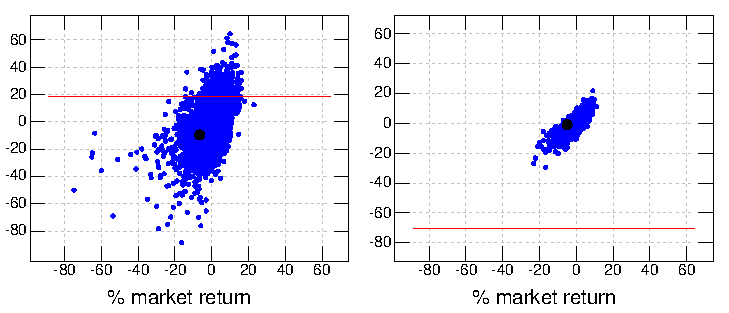
\includegraphics{simulation.pdf}
\caption{Six thousand simulated bivariate 1 month forward returns for CBA and the market at start of January 2009 (left panel)  and December 2014 (right panel). Note scales in both panels are the same, the relatively large volatility in the left panel, and the left skew in the  marginal distributions.}
\label{simulation}
\end{center}
\end{figure}

While the above discussion suggests the, as is obvious after the fact, that December 2009 the CBA bank was under much stress the above calculations do not actually reflect the reflect the real stress.   In terms of the development of the previous sections the actual stress is beta given a stressor function $\phi$ and stressor variable.   In this case the stressor variable is the market return, on the horizontal axis in each panel.   Stress occurs if the market return is low.   In the left panel low market outcomes are likely to lead to sharply lower CBA bank returns, as compared to the right panel.   This is suggested by the slope of the scatter plots:  the left slope appears steeper than the right and hence any stress in the market -- in the sense of a market downturn is expected to lead to a larger drop in the CBA bank return in the left scenario as compared to the right scenario.   The magnitudes of the two responses depends on the stressor function.   In essence the stressor function formalises the notion as to what constitutes a ``big" drop.   If a big drop is the expected worst in 20 similar market scenarios then the stress in the left and right are xxx and xxx, respectively.        



\section{Application to Australian financial institutions}

In this study we consider financial data for  the 8 Australian banks.

\begin{table}[htdp]
\caption{Four major and four minor Australian banks}
\begin{center}
\begin{tabular}{l|l}
\hline
cba & Commonwealth Bank of Australia\\
anz & Australia \& New Zealand Bank\\
nab & National Australia Bank\\
wbc & Westpac Banking Corporation\\
\hline
mqg & Macquarie Banking Group\\
boq & Bank of Queensland\\
ben & Bendigo and Adelaide Bank\\
aba & Auswide Bank\\
\hline
\end{tabular}
\end{center}
\label{banks}
\end{table}%


The analysis is based on daily return data is collected from   3 April 2000 through to 1 December 2014 for a total of  3848 trading days.
Prices, adjusted for dividends are plotted in \fref{prices}.

\begin{figure}[htbp]
\begin{center}
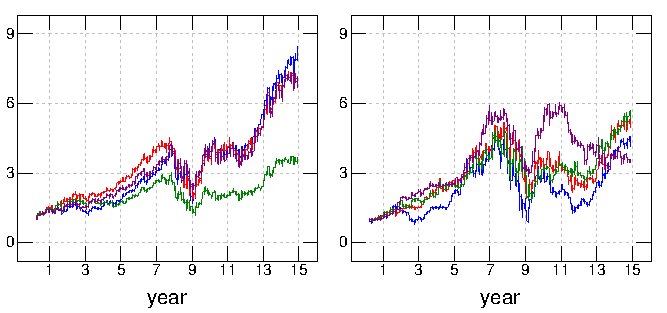
\includegraphics{prices.pdf}
\caption{Basel log--leverages for four major (left panel) and four minor (right panel) Australian banks from April 2000 through to December 2014.  Note all banks suffer  falls starting the middle of 2008.}
\label{prices}
\end{center}
\end{figure}
 
At each of the first trading day in the months from January 2003 through to December 2014,  all prior returns are used estimate a TARCH-DCC model described below.   For each first trading day of the month, the fitted model is then used to simulate the forward return distribution over the next 22 trading days, corresponding to approximately one month.  The details of the fitted models are described in the next subsection.



\subsection{Forward return simulation}

The forward simulations are implemented similar to \cite{brownlees2015}.   Given the latest available volatility and correlation estimates the filter recursions are moved forward in time using innovations randomly chosen from past standardised innovations.  Thus the innovations are chosen to have the same marginal distributions as applicable in the past.  The random choices are such  that the same market return innovations are used in each bivariate analysis.   



\subsection{Systemic beta's}

\fref{Bbeta} displays the system systemic beta (left panel) and the firm specific systemic beta's (right panel)  for each month from January 2003 through to December 2014.   The stressor is the ASX market return while the stressor function is the expected worst outcome in $n=12$ identical scenarios:  $\phi(u)=n(1-u)^{n-1}$.

\begin{figure}[htbp]
\begin{center}
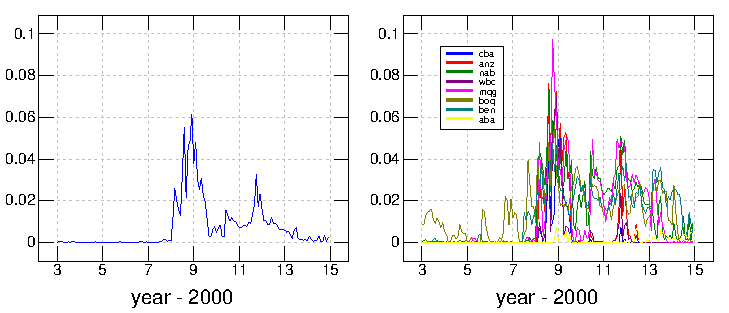
\includegraphics{Bbeta.pdf}
\caption{Systemic beta's.  The left panel displays the system systemic beta.   The right panel indicates systemic beta's for each of the eight banks.  In each case the stressor is market return and the stress function is the expected worst outcome in 12 identical scenarios.}
\label{Bbeta}
\end{center}
\end{figure}

The left panel of \fref{Bbeta} indicates that up to about late 2008, there was no system systemic stress:  The chance of a Basel default was virtually zero.   However, indicated in the right panel, the BOQ bank did have have substantial systemic risk -- ie a substantial risk of sliding into Basel default under the systemic stress of a broad market downturn.

\subsection{Stressors}

Two different stressors are used:   



\section{Standardised SRISK and layer dependence}

Standardising SRISK by subtracting the unconditional expected capital shortfall and dividing by the same assuming maximum systemic risk yields a quantity which is independent of initial debt and equity. In addition standardised SRISK reflects the local dependence between an individual firm and the market at the selected threshold of the systemic event. Hence varying the threshold yields the dependence structure of individual firm and market returns from benign events all the way to tail events.

The unconditional expected capital shortfall for firm $i$ is $\E(c_i)=kd_i-(1-k)w_i\{1+\E(r_i)\}$, suggesting the standardised SRISK
$$
\mathrm{SRISK}_i^* \equiv \frac{\mathrm{SRISK}_i-\E(c_i)}{\max(\mathrm{SRISK}_i)-\E(c_i)}
=\frac{\E(r_i)-\E(r_i|u_m<a)}{\E(r_i)-\E(r_i|u_i<a)}
$$
$$
=\frac{\cov\{r_i,\overline{I}_a(u_m)\}}{\cov\{r_i,\overline{I}_a(u_i)\}}
=\frac{\cov\{r_i,I_a(u_m)\}}{\cov\{r_i,I_a(u_i)\}} 
$$
where $\overline{I}_a(z)\equiv (z<a)$ and $I_a(z)\equiv (z>a)$ are indicators. Maximum SRISK occurs if firm return is comonotonic with the market return or $u_i=u_m$, $u_i$ being the percentile rank of $r_i$. Standardised SRISK is hence layer dependence on the original scale, and mainly lies between 0 and 1 indicating independence and comonotonicity, respectively. Varying $a$ reveals the local dependence between firm and market returns at different thresholds, with $a\rightarrow 0$ yielding the lower extreme tail dependence in a market crash of maximum severity.

Performing the same standardising on $\widetilde{\mathrm{SRISK}}_i$ which is a weighted average of SRISK for firm $i$ across various thresholds yields
$$
\widetilde{\mathrm{SRISK}}_i^* = \frac{\cov\{r_i,\phi(u_m)\}}{\cov\{r_i,\phi(u_i)\}}   \;.
$$





\section{Comparing SRISK for different firms (not sure)}

Suppose of interest is whether $\beta_{it}$ varies similarly  across firms as $\tau$ varies where $\tau$ is the threshold, $k$, or some other parameter used to compute $\beta_{it}$. High correlation implies high systemic risk since firms are simultaneously affected.

Define $\eps_{it}\equiv(\phi-1)p_{it}$ and $\eps_{it}$ as the vector with components $\eps_{it}$.  Then $\E(\eps_{it}|\tau)=\sigma_\phi(\tau)\beta_{it}(\tau)$, the stress in firm $i$ at the given parameter setting $\tau$  and
$$
\cov\{\E(\eps_{it}|\tau)\}=\cov(\eps_{t})-\E\{\cov(\eps_{it}|\tau)\}\ ,
$$
is the covariance between stresses as $\tau$, the stress parameter varies.   Thus the covariances and correlations between firms as stress parameters vary can be computed from the covariability between the $\eps_{it}$ and the ...

\begin{comment}
\subsection{Weihao - Allocating the market put}

The overall market shortfall after allowing for diversification between firms is
$$
p_{mt}\equiv k_+ |1-\e^{-\ell^*_{mt}+\nu_{mt}}|^+
= k_+|\Ex (1-\e^{-\ell^*_{it}+\nu_{it}})|^+
=I(\nu_{mt}<\ell_{mt}^*)k_+\Ex(1-\e^{-\ell^*_{it}+\nu_{it}}) 
$$
and hence the portion attributable to firm $i$ is $k_i(1-\e^{-\ell^*_{it}+\nu_{it}}) I(\nu_{mt}<\ell_{mt}^*)$, its capital shortfall or surplus when the overall market is in a shortfall. The allocation of the stressed expectation $\E(p_{mt})$ is then
$$
k_i\E\{(1-\e^{-\ell^*_{it}+\nu_{it}}) I(\nu_{mt}<\ell_{mt}^*)\}
$$
and applying $\Ex$ to the above expression yields $\E(p_{mt})$.
\end{comment}

\section{Standardised SRISK and layer dependence}

Standardising SRISK by subtracting the unconditional expected capital shortfall and dividing by the same assuming maximum systemic risk yields a quantity which is independent of initial debt and equity. In addition standardised SRISK reflects the local dependence between an individual firm and the market at the selected threshold of the systemic event. Hence varying the threshold yields the dependence structure of individual firm and market returns from benign events all the way to tail events.

The unconditional expected capital shortfall for firm $i$ is $\E(c_i)=kd_i-(1-k)w_i\{1+\E(r_i)\}$, suggesting the standardised SRISK
$$
\mathrm{SRISK}_i^* \equiv \frac{\mathrm{SRISK}_i-\E(c_i)}{\max(\mathrm{SRISK}_i)-\E(c_i)}
=\frac{\E(r_i)-\E(r_i|u_m<a)}{\E(r_i)-\E(r_i|u_i<a)}
$$
$$
=\frac{\cov\{r_i,\overline{I}_a(u_m)\}}{\cov\{r_i,\overline{I}_a(u_i)\}}
=\frac{\cov\{r_i,I_a(u_m)\}}{\cov\{r_i,I_a(u_i)\}} 
$$
where $\overline{I}_a(z)\equiv (z<a)$ and $I_a(z)\equiv (z>a)$ are indicators. Maximum SRISK occurs if firm return is comonotonic with the market return or $u_i=u_m$, $u_i$ being the percentile rank of $r_i$. Standardised SRISK is hence layer dependence on the original scale, and mainly lies between 0 and 1 indicating independence and comonotonicity, respectively. Varying $a$ reveals the local dependence between firm and market returns at different thresholds, with $a\rightarrow 0$ yielding the lower extreme tail dependence in a market crash of maximum severity.

Performing the same standardising on $\widetilde{\mathrm{SRISK}}_i$ which is a weighted average of SRISK for firm $i$ across various thresholds yields
$$
\widetilde{\mathrm{SRISK}}_i^* = \frac{\cov\{r_i,\phi(u_m)\}}{\cov\{r_i,\phi(u_i)\}}   \;.
$$




\subsection{Contagion effects}
Definition \eref{nsrisk} can be generalized to capture contagion effects.  Consider 
\be{cont}
\Ex^j\{\E^j(p_{it})\}=\E^j\{\Ex^j(p_{it})\}\ ,
\ee
where  $\E^j$ denotes the stressed conditional expectation, conditioning on a firm $j$ breach, and $\Ex^j$ is an debt weighted average excluding firm $j$.  Firm $j$ is systemically important  if a Basel breach in firm $j$ leads to large increase in system systemic risk
$$
c_{ij}\equiv \frac{\E^j\{\Ex^j(p_{it})\}}{\E\{\Ex(p_{it})\}}-1\ .
$$

\subsection{Diversification effects} 

Suppose debt and equity are  aggregated across firms to yield $d_t$ and $w_t$.  The system log leverage is  
$$
\ell_t =  \ln \frac{d_t}{w_t} =  \ln \sum_i\frac{w_{it}}{w_t}\frac{ d_{it}}{ w_{it}} = \ln \Ex_w(\e^{\ell_{it}}) \ ,
$$
where $\Ex_w$ denotes an equity weighted average.  A system wide breach of the Basel II limit occurs at $t+h$ if
$
\nu_t < \ell_t^*\equiv \ell_t - 2.44
$
where $\nu_t$ is the rate of return on total equity $w_t$:
\be{ew}
 \nu_t = \ln \frac{w_{t+h}}{w_t} = \ln \Ex_w\left(\frac{w_{i,t+h}}{w_{it}}\right) = \ln \Ex_w(\e^{\nu_{it}})\ . 
\ee

Similar to before define a put for the system and its (stressed) expected value
$$
p_t\equiv k|1-\e^{\nu_t-\ell_t^*}|^+\cq \Es(p_t)\le\Ex\{\Es(p_{it})\}\ .
$$
The inequality is a result  of diversification effects:   low liquidity  in one firm is implicitly offset by high liquidity  in other  firms.


\section*{Appendix}

Denote the daily (log) return as
\newcommand{\vareps}{\varepsilon}
\be{mean.model}
\delta_{it}=\mu+\sigma_{it}\ep_{it}s_{it}\cq \eps_{it}\sim (0,1)\cq  \eps^-_{it}\equiv I(\eps_{it}<0)=I(\delta_{it}<\mu)\ ,
\ee
Thus returns are assumed to have an unconditionally constant mean.   The notation $\eps_{it}^-$ indicates whether there is a negative return:  $I$ denoting the indicator function.  The volatility is modelled with the TARCH model
\be{vol}
\sigma_{t+1}^2 = \omega+ \sigma^2_{it}\{\beta+(\alpha+\gamma \eps^-_{it})\eps_{t}^2\}\\ .
\ee
Hence the response of the variance to $\eps_{it}^2$  is increased by $\gamma$   if $\eps_{i_{it}t}<0$ compared to the response if $\eps_{it}>0$.  This is a simple threshold GARCH model:  called TARCH.   In the fits it is assumed the mean $\mu$ does not vary with time $t$ and the single lag in both the $\sigma_{it}^2$ and $\eps_{it}$ is sufficient to capture the dynamics of volatility. 

The model \eref{mean.model} and \eref{vol} is fit  for each security $i$ including the market,  $i=m$.   The correlations between securities and the market are also modelled using  positive definite recursions   \citep{engle2002dynamic}
$$
(Q_{t+1}-S) = \alpha (\eta_{it}\eta_{it}'-S) + \beta (Q_{it}-S)\cq \eta_{it}\equiv(\eps_{it},\eps_{mt})' ,
$$
A   Dynamic Conditional Correlation (DCC) model is estimated for  firm and market returns.  Write
\newcommand{\veps}{\varepsilon}
$$
\cov (\delta_{it}|t) = V_{it}R_{it}V_{it}'\cq R_{it}\equiv \cov(\veps_{it}|t)\cq \veps_{it}=V_{it}^{-1}\delta_{it}\ ,
$$
where $R_{it}$ and  $V_{it}$  are the correlation and diagonal volatility matrix, respectively, at time $t$.   Volatilities in $V_{it}$  are estimated using univariate threshold GARCH models.  The estimate of $R_{it}$ corresponds to the correlations in covariance matrix $C_{it}$ assuming
$$
(C_{it} - C) = \alpha (C_{t-1}-C)+\beta (\veps_{it}\veps'_{it}-C) \cq C\equiv\cov(\veps_{it})\ .
$$
where $C$ is the long run covariance matrix.




\section*{References}
\bibliography{/users/pietdejong/documents/research/cifr/piet2}

\end{document}
